%%%%%%%%%%%%%%%%%%%%%%%%%%%%%%%%%%%%%%%%%%%%%%%%%%%
%% P3: Phenomenology of Particle Physics                         
%%
%% Author:  André Rubbia                   		 
%%
%% Figure 1.4 Effect of the discrete symmetries on an electron or positron
%%
%% This work is licensed under the Creative Commons Attribution 4.0 International License. 
%% To view a copy of this license, visit http://creativecommons.org/licenses/by/4.0/ or 
%% send a letter to Creative Commons, PO Box 1866, Mountain View, CA 94042, USA.
%%
%%%%%%%%%%%%%%%%%%%%%%%%%%%%%%%%%%%%%%%%%%%%%%%%%%%

\documentclass[a4paper,10pt]{article}

\usepackage[T1]{fontenc}
\usepackage[utf8]{inputenc}
\usepackage{lmodern}
\usepackage[labelfont=bf]{caption}

\usepackage{tikz}
\usetikzlibrary{patterns}
\usetikzlibrary{decorations.pathmorphing}
\usetikzlibrary{decorations.markings}
\usetikzlibrary{arrows}
\usetikzlibrary{svg.path}
\usetikzlibrary{shapes}
\usetikzlibrary{arrows.meta}
% define the arrow style
\tikzset{
    arrow/.style={
        decoration={
            markings,
            mark=at position .5 with {
                \arrow[#1, scale=1.5]{latex}
            }
        },
        postaction={decorate},
    }
}
\tikzset{
    arrow flipped/.style={
        decoration={
            markings,
            mark=at position .5 with {
                \arrow[#1, scale=1.5]{latex reversed}
            }
        },
        postaction={decorate},
    }
}
\pgfkeys{/pgf/number format/.cd,1000 sep={}}

\usepackage{pgfplots}
\pgfplotsset{compat=1.17}
\usepgfplotslibrary{ternary}
\usepgfplotslibrary{fillbetween}
\usepgfplotslibrary{external}

\def\d{\mathrm{d}}

\begin{document}

%%%%%%%%%%%%%%%%   FIGURE  %%%%%%%%%%%%%%%%%%%%%%%%%%%%%%
\begin{figure}[htb]
\begin{center}
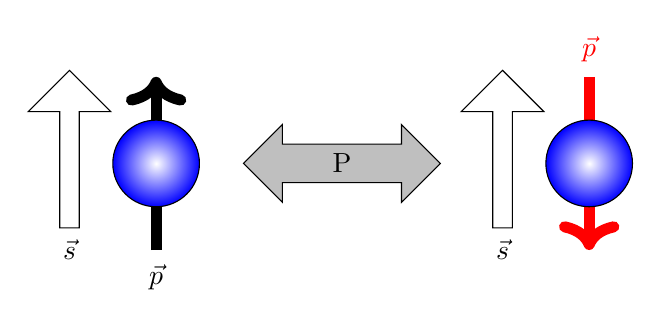
\begin{tikzpicture}[scale=1.1]
 \begin{scope}[shift={(-2,0)}]
\draw[line width=4pt,black,->] (0,-1) node[below] {$\vec p$} -- (0,1);
\shadedraw[inner color=white, outer color=blue, draw=black] (0,0) circle (0.5cm);
\node[draw, single arrow,
              minimum height=20mm, minimum width=8mm,
              single arrow head extend=4mm,
              anchor=west, rotate=90] at (-1,-0.75) {$$};
\node at (-1,-1) {$\vec s$};
\end{scope}
\node[draw, fill=lightgray,double arrow,
              minimum height=25mm, minimum width=8mm,
              single arrow head extend=4mm,
              anchor=west, rotate=0] at (-1,0) {P};
 \begin{scope}[shift={(3,0)}]
\draw[line width=4pt,red,->] (0,1) node[above] {$\vec p$} -- (0,-1);
\shadedraw[inner color=white, outer color=blue, draw=black] (0,0) circle (0.5cm);
\node[draw, single arrow,
              minimum height=20mm, minimum width=8mm,
              single arrow head extend=4mm,
              anchor=west, rotate=90] at (-1,-0.75) {$$};
\node at (-1,-1) {$\vec s$};
\end{scope}
\end{tikzpicture}\\

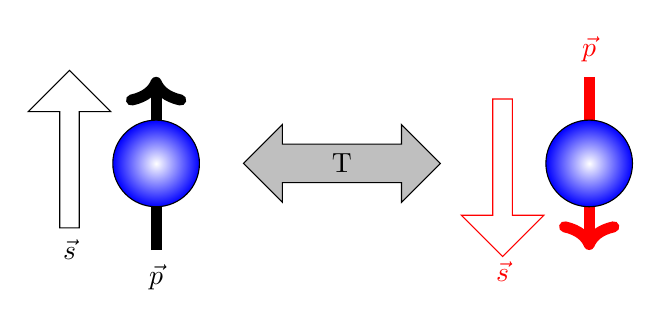
\begin{tikzpicture}[scale=1.1]
 \begin{scope}[shift={(-2,0)}]
\draw[line width=4pt,black,->] (0,-1) node[below] {$\vec p$} -- (0,1);
\shadedraw[inner color=white, outer color=blue, draw=black] (0,0) circle (0.5cm);
\node[draw, single arrow,
              minimum height=20mm, minimum width=8mm,
              single arrow head extend=4mm,
              anchor=west, rotate=90] at (-1,-0.75) {$$};
\node at (-1,-1) {$\vec s$};
\end{scope}
\node[draw, fill=lightgray,double arrow,
              minimum height=25mm, minimum width=8mm,
              single arrow head extend=4mm,
              anchor=west, rotate=0] at (-1,0) {T};
 \begin{scope}[shift={(3,0)}]
\draw[line width=4pt,red,->] (0,1) node[above] {$\vec p$} -- (0,-1);
\shadedraw[inner color=white, outer color=blue, draw=black] (0,0) circle (0.5cm);
\node[draw, color=red, single arrow,
              minimum height=20mm, minimum width=8mm,
              single arrow head extend=4mm,
              anchor=west, rotate=-90] at (-1,0.75) {$$};
\node[red] at (-1,-1.25) {$\vec s$};
\end{scope}
\end{tikzpicture}\\
\vspace{0.5cm}
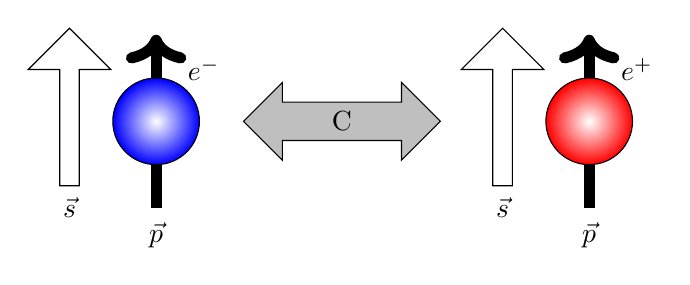
\begin{tikzpicture}[scale=1.1]
 \begin{scope}[shift={(-2,0)}]
\draw[line width=4pt,black,->] (0,-1) node[below] {$\vec p$} -- (0,1);
\shadedraw[inner color=white, outer color=blue, draw=black] (0,0) circle (0.5cm);
\node[draw, single arrow,
              minimum height=20mm, minimum width=8mm,
              single arrow head extend=4mm,
              anchor=west, rotate=90] at (-1,-0.75) {$$};
\node at (-1,-1) {$\vec s$};
\node at (0.55,0.6) {$e^-$};
\end{scope}
\node[draw, fill=lightgray,double arrow,
              minimum height=25mm, minimum width=8mm,
              single arrow head extend=4mm,
              anchor=west, rotate=0] at (-1,0) {C};
 \begin{scope}[shift={(3,0)}]
\draw[line width=4pt,black,->] (0,-1) node[below] {$\vec p$} -- (0,1);
\shadedraw[inner color=white, outer color=red, draw=black] (0,0) circle (0.5cm);
\node[draw, single arrow,
              minimum height=20mm, minimum width=8mm,
              single arrow head extend=4mm,
              anchor=west, rotate=90] at (-1,-0.75) {$$};
\node at (-1,-1) {$\vec s$};
\node at (0.55,0.6) {$e^+$};
\end{scope}
\end{tikzpicture}\\
\caption{Effect of the discrete symmetries $P$ (top), $T$ (middle), and $C$ (bottom) on an electron or positron. Note that the action of the operator applied on the state twice results in the original particle.}
\label{fig:effectdiscreteonparticle}
\end{center}
\end{figure}
%%%%%%%%%%%%%%%%  END FIGURE  %%%%%%%%%%%%%%%%%%%%%%%%%%%%%%
%
\end{document}
